\section{Оптимизация разноцветных ящиков.}
\textbf{Серый ящик} представляет собой какое-то абстрактное логическое вычислимое нечто (какая-либо операция, программа, продукт), и мы частично знаем, что является краеугольным механизмом для порождения этих самых вычичлений.
Оптимизатор - некоторая функция, можем знать характер этой функции, возможно знаем значения, которые претендуют на звание локального оптимума.

\textbf{Белый ящик} - известно все.

\textbf{Черный ящик} - неизвестно ничего. Оптимизатор - некоторая функция, которая принимает на вход аргументы, не знаем ничего о ней.

\textbf{Gray Box Optimization в широком контексте}
\begin{itemize}
    \item Случайный поиск
    \begin{itemize}
        \item Почти ничего не знаем; надеемся на лучшее значение критерия
    \end{itemize}
     \item Локальный поиск
    \begin{itemize}
        \item Надеемся на локальность; получаем локальные оптимумы, нам этого достаточно
    \end{itemize}
     \item Black-Box Optimization(метаэвристики)
    \begin{itemize}
        \item Надеемся на наличие у задачи структуры; больше времени тратим получаем решение лучше
    \end{itemize}
    \item Gray-Box Optimization
    \begin{itemize}
        \item Знаем структуру задачи; надеемся, что неизвестные части задачи не слишком велики т.е. их можно нати и выразить некоторой функцией за адекватное время
    \end{itemize}
\end{itemize}

\begin{figure}[h]
    \centering
    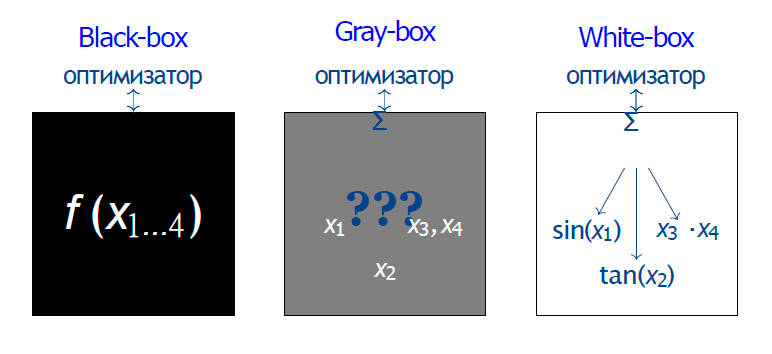
\includegraphics[width=0.8\linewidth]{images/colorbox.PNG}
% \end{figure}
    
% \begin{figure}[h]
%     \centering
    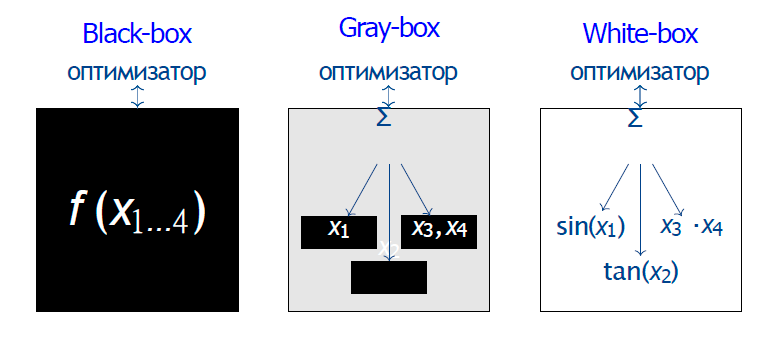
\includegraphics[width=0.8\linewidth]{images/colorbox2.PNG}
\end{figure}

\textbf{Gray-Box Optimization для псевдобулевых функций}\\
Общий вид псевдобулевых функций в контексте Gray Box optimization\\
У нас есть некоторый оператор, функции, зависящие от некоторого набора аргументов. Значение функций - комбинация 0 и 1, по которым строится битовая маска. т.е. итовая строка значений серого ящика.
\begin{figure}[h]
\centering
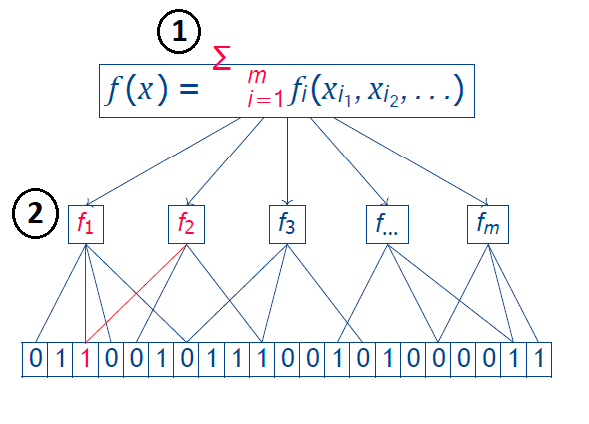
\includegraphics[width=0.45\linewidth]{images/colorbox3.PNG}
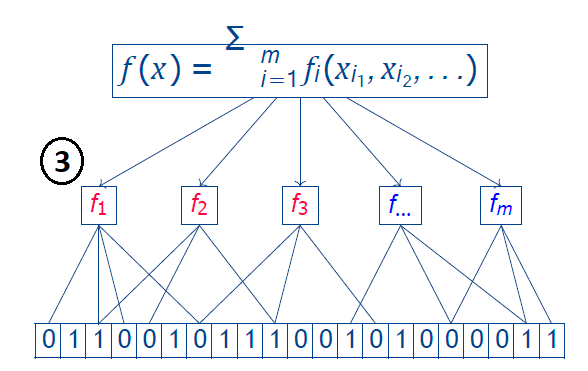
\includegraphics[width=0.45\linewidth]{images/colorbox4.PNG}
\end{figure}
\begin{enumerate}
    \item Сумма может заменяться на другие способы агрегации. В зависимости от того, обратима ли агрегация или нет, могут быть спецэффекты. Может быть случайный выбор, объединение по какому-либо критерию. Ключевой фактор выбора оператора агрегации - его обратимость
    \item Различные подфункции могут зависеть от одних и тех же переменных
    \item Группы переменных могут оказаться независимыми. В данном примере красные и синие функции могут оптимизироваться независимо\\
    \item Функция называется \textbf{k-ограниченной} если каждая ее подфункция зависит от не более чем k переменных. Еще одно название:\textbf{ Mk ландшафт}\\ Если есть некоторое ограничение на функцию, то легче заниматься оптимизацией черного ящика.
\end{enumerate}
Зачем заниматься оптимизацией серого ящика? - Большинство задач не имеют четкого задания структур. Как правило - это полуабстрактное описание взаимодействия с представителями той или иной контектной среды. Мы понимаем зависимость между объектами и резльтатами, но установить характер того как она устроена изнутри не представляется возможным. \\
Пример: задачи по подбору хеш-функций, которые встроены в единый механизм критой системы. Оценка криптосистем при утечке информации изнутри.
